% Chapter 1
\chapter{مقدمه}

\section{بیان مسئله و ضرورت پژوهش}

در صنایع بزرگ، عدم اطلاع از شرایط عمر مفید تجهیزات، ماشین‌آلات و دستگاه‌های صنعتی باعث خرابی‌های ناگهانی آن‌ها می‌شود و این امر به عنوان یکی از چالش‌های اصلی صنایع مختلف، قابل بررسی است. خرابی‌های ناگهانی در این صنایع، می‌تواند عملیات را مختل کند، هزینه‌های نگهداری را افزایش دهد و حتی ایمنی را به خطر بیندازد. این مشکلات بیشتر ناشی از رویکردهای سنتی نگهداری و تعمیر است که نمی‌تواند با پیچیدگی‌ و پویایی موجود در داده‌ها نتیجه مطلوبی داشته باشد\cite{ismail2025systematic}.


امروزه، دستگاه‌های صنعتی، چه در کارخانه‌های تولیدی، تأسیسات انرژی یا شبکه‌های حمل و نقل، با طول عمر مورد انتظار حدود ۱۰ سال مهندسی می‌شوند \cite{aivaliotis2021degradation}.
 با این حال، قرار گرفتن در معرض تأثیرات مخرب و مداوم مانند اضافه بار، آب و هوای نامناسب، فرسودگی مواد و دیگر تغییرات محیطی، به تدریج این دارایی‌ها تخریب شده و منجر به خرابی‌ها و وقفه‌های غیرمنتظره می‌شود به طوری که عمر مفید آن‌ها بسیار کمتر از عمر مورد انتظار واقع می‌گردد.
  طبق گزارش‌های ارائه شده، خرابی قطعات مهندسی در صنایع مختلف، بین سال‌های ۲۰۱۰ تا ۲۰۱۸، ۴۰ درصد افزایش یافته است \cite{corchado2019failure}. علاوه بر این، تنها یک روز خرابی برنامه‌ریزی نشده می‌تواند بین ۱۰۰۰۰۰ تا ۲۰۰۰۰۰ یورو هزینه غیر قابل پیش‌بینی داشته باشد \cite{mathur2001reasoning}.
  
ضرورت پژوهش در این حوزه از آنجایی ناشی می‌شود که صنایع نه تنها برای پیشرفت و توسعه، بلکه برای بقا، نیاز به بهبود کارایی و کاهش هزینه‌ها و خطر‌های خود دارند. فناوری دوقلوهای دیجیتال به عنوان یک راه‌حل نوین، امکان ارائه دوقلوی دیجیتال برای تجهیزات را فراهم می‌کند تا خرابی‌ها را پیش‌بینی و مدیریت کند و بهترین‌ زمان را برای بررسی و تعمیر آن‌ها ارائه دهد\cite{tao2019digital}.
 دوقلوهای دیجیتال با ایجاد مدل‌های دیجیتال پویا در هر لحظه از موجودیت‌های فیزیکی و استفاده از تجزیه و تحلیل داده‌های حسگرها و سیستم‌های عملیاتی، امکان تصمیم‌گیری بهتر را فراهم می‌کند\cite{vandinter2022predictive}. 
 این رویکرد، با ادغام هوش مصنوعی به خصوص، یادگیری عمیق، نه تنها به شناسایی سریع‌تر مشکلات کمک می‌کند، بلکه الگویی برای صنایع متنوع ارائه می‌دهد تا از عواقب منفی خرابی‌ها جلوگیری شود\cite{lv2024artificial} \cite{kreuzer2024artificial}. همچنین ادغام آن با مدل‌های زبانی بزرگ، امکان تعامل هر چه ساده‌تر با دوقلو‌های دیجیتال ایجاد می‌شود و می‌توان به وسیله زبان طبیعی، درباره موجودیت‌های فیزیکی پرس‌وجو کرد یا دستوراتی برای اعمال بر آن‌ها داد\cite{CHEN2025102982LLMDT}.
  
  پژوهش حاضر با تمرکز بر چارچوب چندعاملی در دوقلوهای دیجیتال و معماری لایه‌ای در آن و در نظر گرفتن ادغام با یادگیری عمیق و مدل‌های زبانی بزرگ، به دنبال ارائه راه‌حلی عمومی برای دستگاه‌های صنعتی است تا مدیریت نگهداری را به سطحی هوشمند و تعاملی، ارتقا دهد.
  
  
  
\section{اهمیت پژوهش}

پیش‌بینی خرابی و پایش بی‌درنگ تجهیزات در صنایع، نقش کلیدی در افزایش ایمنی، کارایی و پایداری عملیات ایفا می‌کند، زیرا امکان اقدامات پیشگیرانه را فراهم می‌آورد و از وقوع شکست‌های پرهزینه جلوگیری می‌نماید.
 اهمیت این پژوهش در ادغام مدل‌های پیشرفته یادگیری عمیق و مدل‌های زبانی بزرگ در چارچوب دوقلوهای دیجیتال نهفته است، که نه تنها عمر مفید تجهیزات را بهبود می‌بخشد، بلکه دلایل احتمالی خرابی را توضیح می‌دهد و تصمیم‌گیری‌های هوشمند را تسهیل می‌کند.
  در سطح گسترده‌تر، این رویکرد می‌تواند عملیات را بهینه‌سازی کند و نرخ در دسترس بودن تجهیزات را افزایش دهد، که در صنایع مانند تولید، انرژی و حمل‌ونقل، تحول‌آفرین است. 
  مقالات اخیر تأکید دارند که دوقلوهای دیجیتال، با شبیه‌سازی فرایند‌های واقعی و تحلیل داده‌های بزرگ، به مدیریت فعال خرابی‌ها کمک می‌کنند و پایه‌ای برای نوآوری‌های آینده در ادغام هوش مصنوعی با سیستم‌های صنعتی فراهم می‌آورند. این کار نه تنها مسائل عملی را حل می‌کند، بلکه کاربردپذیری آن در صنایع گوناگون، اهمیت استراتژیک آن را برجسته می‌سازد.


روش‌‌های نگهداری از دستگاه‌ها و ابزار‌های صنعتی در را می‌توان به سه دسته تقسیم کرد\cite{ismail2025systematic}: 

\begin{enumerate}
	\item 
\gls{reactive maintenance}، به این معنی که تعمیر یک دستگاه، پس از خراب شدن و از کار افتادن آن انجام شود که منجر به در دسترس نبودن آن برای مدت زمان طولانی شده و هزینه‌های غیرقابل پیش‌بینی را تحمیل می‌کند.
	\item 
\gls{preventive maintenance}، که شامل نگهداری برنامه‌ریزی شده در فواصل زمانی ثابت بدون توجه به وضعیت واقعی تجهیزات است. اگرچه این روش خرابی‌های ناگهانی را کاهش می‌دهد، اما بیشتر مواقع موجب تعویض زودهنگام قطعات و استفاده نابهینه از منابع می‌شود.
	\item 
\gls{predictive maintenance}، با استفاده از نظارت مداوم از طریق داده‌های حسگر در هر لحظه و تجزیه و تحلیل پیشرفته داده‌ها، می‌تواند زمان احتمالی وقوع خرابی را پیش‌بینی کند .
همچنین این روش امکان بررسی‌های هدفمند را فراهم می‌سازد و باعث می‌شود میزان خرابی‌ها به حداقل برسد و در نهایت برنامه‌های نگهداری بهینه شود\cite{rojek2023artificial}.
\end{enumerate}

تأکید بر نقش دوقلوهای دیجیتال چندعاملی در کاهش downtime، بهبود بازدهی، و پیشگیری از حوادث (با مثال‌های واقعی مانند سیستم‌های Rolls-Royce در ۲۰۲۵). بحث در مورد پتانسیل ادغام LLM برای تعامل طبیعی و تصمیم‌گیری هوشمند.



%اینگونه به شکل رفرنس دهید (شکل \ref{fig:intro:populationpyramid} را ببینید)، 
%‎\begin{figure}[t!]‎
%	\centering
%	\subfloat[‏]{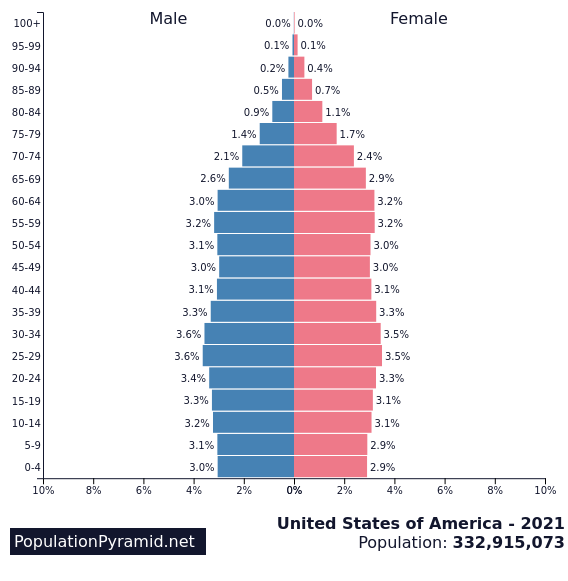
\includegraphics[width=7.25cm]{images/population_data/USA.png}}
%	\qquad
%	\subfloat[]{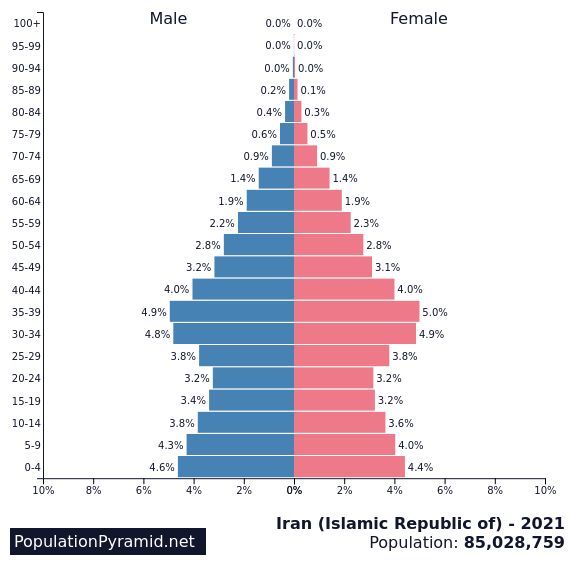
\includegraphics[width=7.25cm]{images/population_data/iran.png}}
%	\caption[عنوان شکل در فهرست اشکال]
%	{مقایسه هرم جمعیتی دو کشور (الف) ایران و (ب) آمریکا }
%	\label{fig:intro:populationpyramid}
%\end{figure} 


\section{اهداف پژوهش}
هدف اصلی: طراحی چارچوب چندعاملی مبتنی بر DT برای پیش‌بینی و پایش موتورهای جت.
اهداف فرعی: پیاده‌سازی معماری ۵ لایه‌ای، ادغام LLM برای کنترل (مانند خاموش/روشن کردن)، ارزیابی با داده‌های CMAPSS، و پیشنهاد کاربردهای صنعتی.
اضافه کردن سؤالات تحقیق: مثلاً "چگونه ادغام MAS و LLM دقت پیش‌بینی RUL را افزایش می‌دهد؟"
 \cite{karimi2020soft, mohammadimohammadabadi}. 


\section{محدودیت‌های پژوهش و مجموعه داده \lr{CMAPSS}}

توضیح مصنوعی بودن داده‌ها اما اعتبار بالای آن (استفاده‌شده در بیش از ۱۰۰۰ مقاله تا ۲۰۲۵)، محدودیت‌های شبیه‌سازی (عدم داده‌های واقعی بی‌درنگ)، و پتانسیل گسترش به سیستم‌های واقعی (مانند ادغام با IoT).

\section{خلاصه فصل‌ها}
توصیف مختصر ساختار پایان‌نامه.
